\chapter{Analysis of Results from the Core Model} \label{chapter-analysis}


\section{The baseline model} 
The two main hypotheses of this thesis are, first,  that the financial sector affects the ownership of housing and the class structure of society, and second that this may have implications for urban productivity. We begin with the first hypothesis. The section of the model that we call the produces demand for land. In the housing market section land agents bid for land. competition between would-be owner-occupiers and investors results in an evolving allocation of ownership of land. The ownership pattern determines the distribution of the locational rents generated by the city.

\begin{figure}
\centering
\begin{tikzpicture}
  \node at (0,0) (1) {URBAN/PRODUCTION PLATFORM};
   \node[above=1mm of 1] (A1) {$\uparrow$};
   \node[above=1mm of A1] (Pop) {POPULATION};
   \node[above=1mm of Pop] (APop) {$\uparrow$};
   \node[above=1mm of APop]  (3) {BIDS};
   \node[above=1mm of 3] (4) {$\uparrow$};
   \node[above=1mm of 4] (5) {OWNERSHIP};
   \node[above=1mm of 5] (6) {$\uparrow$};
   \node[above=1mm of 6] (7) {RENT DISTRIBUTION};
   \node[above=1mm of 7] (ARent) {$\uparrow$};
    \node [above=1mm of ARent, text width= 6cm, text centered, red] {Tenant sojourner cities\\ Eviction of families from cities\\Growing inequality\\ End of urban home-owning class};
   % \node[above=1mm of 1] (2) {$\uparrow$};
   % \node[above=1mm of 2] (3) {Growing inequality};
   % \node[above=1mm of 3] (4) {$\uparrow$};
   % \node[above=1mm of 4] (5) {Eviction of families from cities};
   % \node[above=1mm of 5] (6) {$\uparrow$};
   % \node[above=1mm of 6] (7) {Tenant sojourner cities};
\end{tikzpicture}
\caption{TODO}
\label{fig:enter-label}
\end{figure}


The interlinked social consequences of any shift from owner-occupancy to tenancy, shown in red, are dramatic. 


%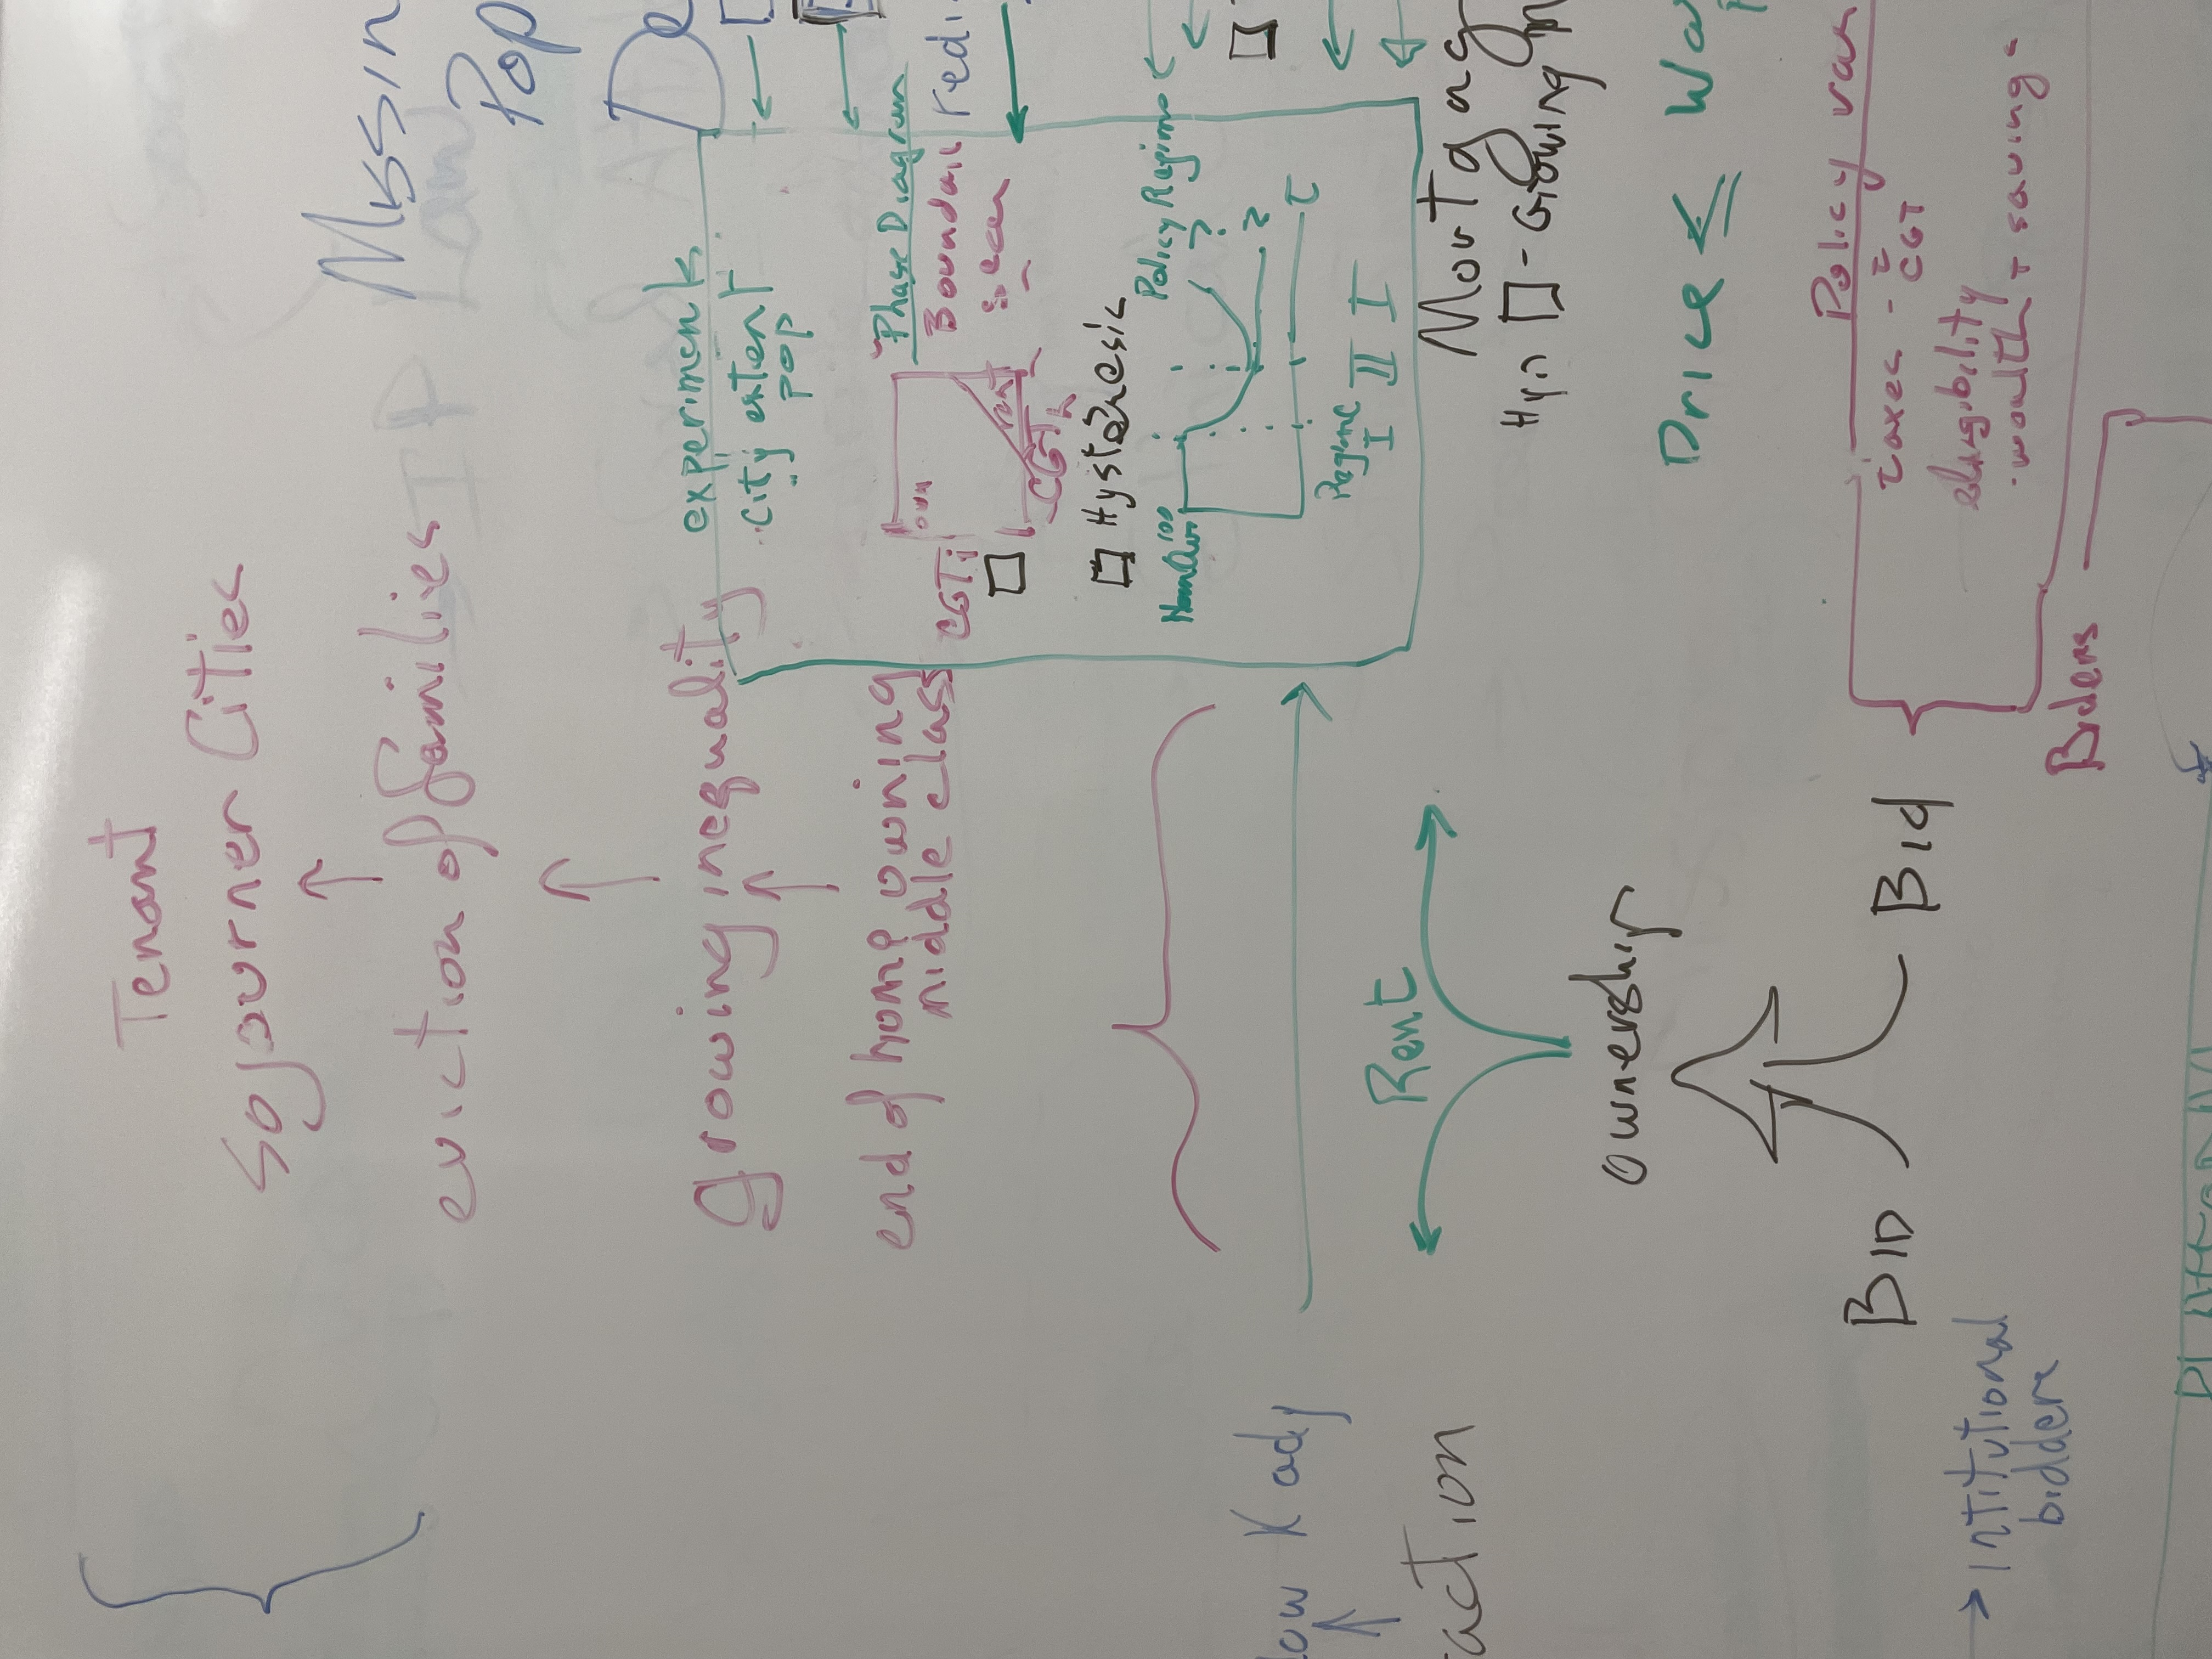
\includegraphics[scale=.5, angle=-90]{fig/IMG_2691.jpg}

We are observing these processes underway in the real world. We need to know if they are explained by a theoretically-consistent model of the urban economy that incorporates the financialization process.

\section{ownership of housing}

With certain plausible parameter settings our baseline model, produces an evolutionary trajectory of class ownership of housing similar to that illustrated in Figure ~\ref{fig:Baseline_ownership_trajectory}. The distribution of ownership then determines the distribution of the locational land rents, which are the product of agglomeration effects. 

Recall that our first hypothesis is that in and \Gls{Alonzo-Jacobs model}, the financial sector will tend to take over a growing share of property ownership within a city. Figure ~\ref{fig:Baseline_ownership_trajectory} shows an initial situation with close to 100 owner-occupiers and a small number of investor-owners. Although the number of owner-occupiers grows in the initial period in Figure ~\ref{fig:Baseline_ownership_trajectory}, over time financial capital acquires an increasing share of the housing stock. By the time the city reaches its maximum size, the city has been transformed from a city of homeowners to a city of tenants.

DISCUSS THE PARAMETERS THAT AFFECT OWNERSHIP? We have conducted parameter sweeps to identify policy parameters that can affect the distribution of ownership.

\begin{figure}
    \centering
    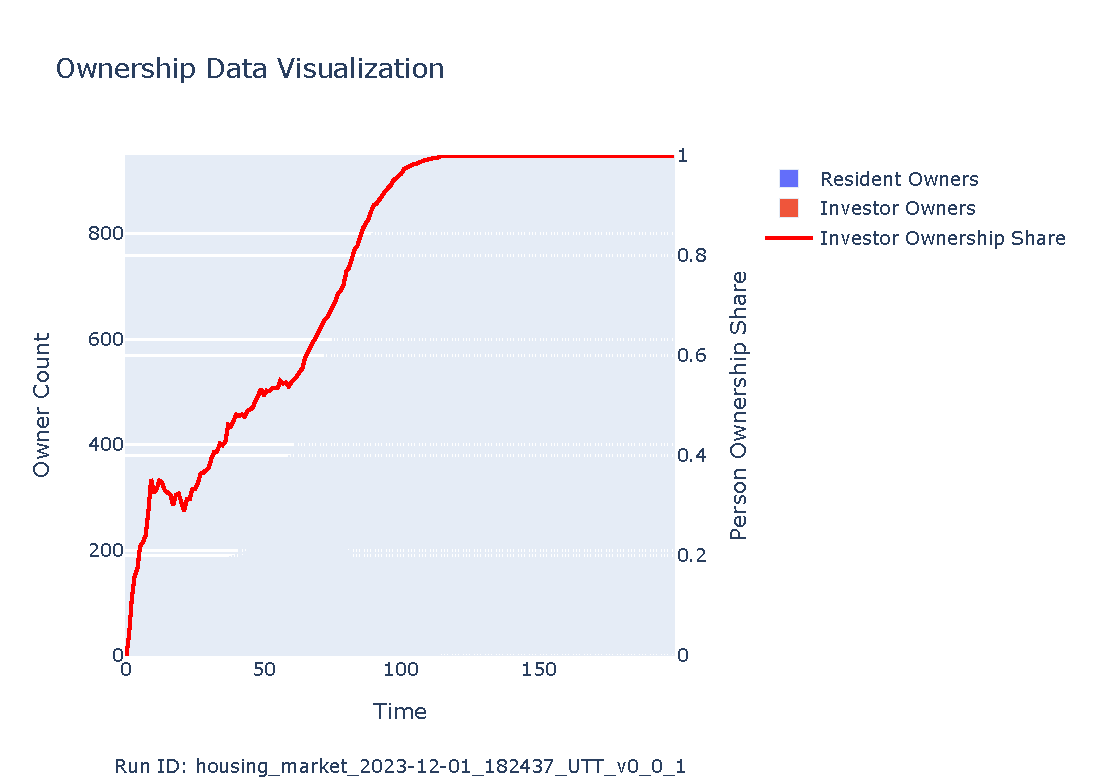
\includegraphics[scale=.8, trim={0 1cm 0 1.8cm},clip]{fig/Analysis/Ownership_Data_1.pdf}
    \caption{The transformation from a city of homeowners to a city of tenants in the baseline model}
    \label{fig:Baseline_ownership_trajectory}
\end{figure}

%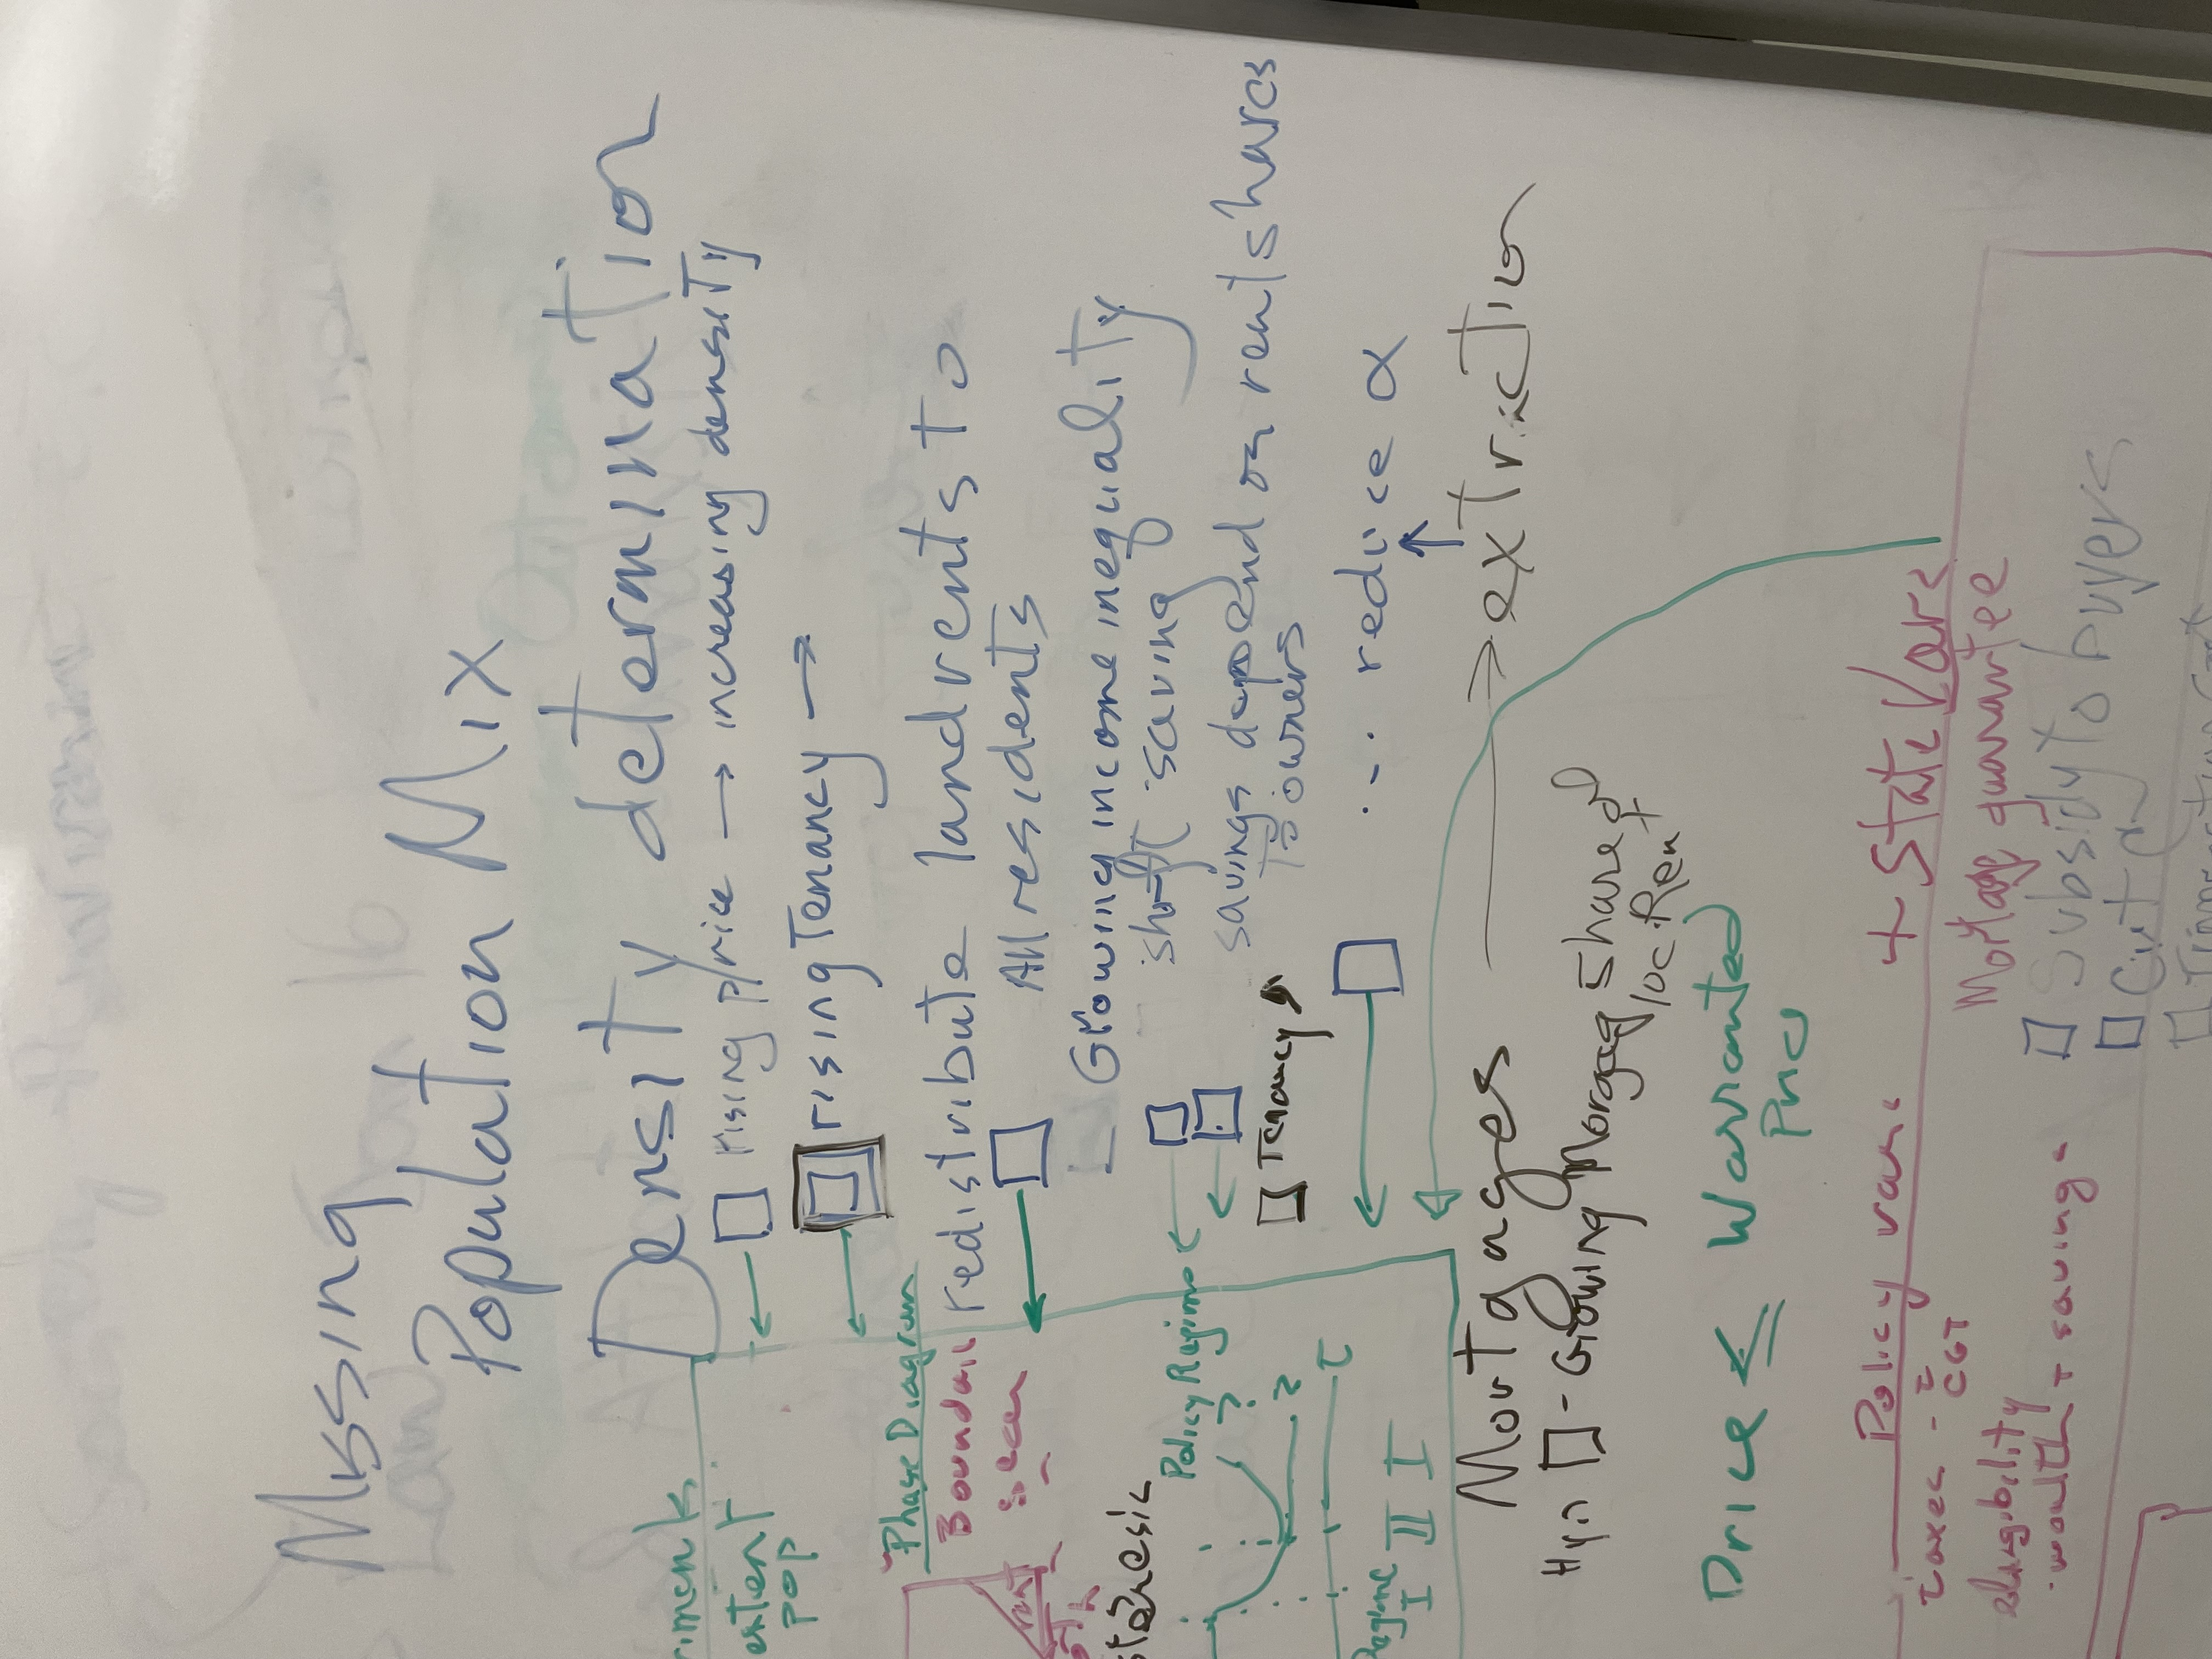
\includegraphics[scale=.5, angle=-90]{fig/IMG_2688.jpg}


%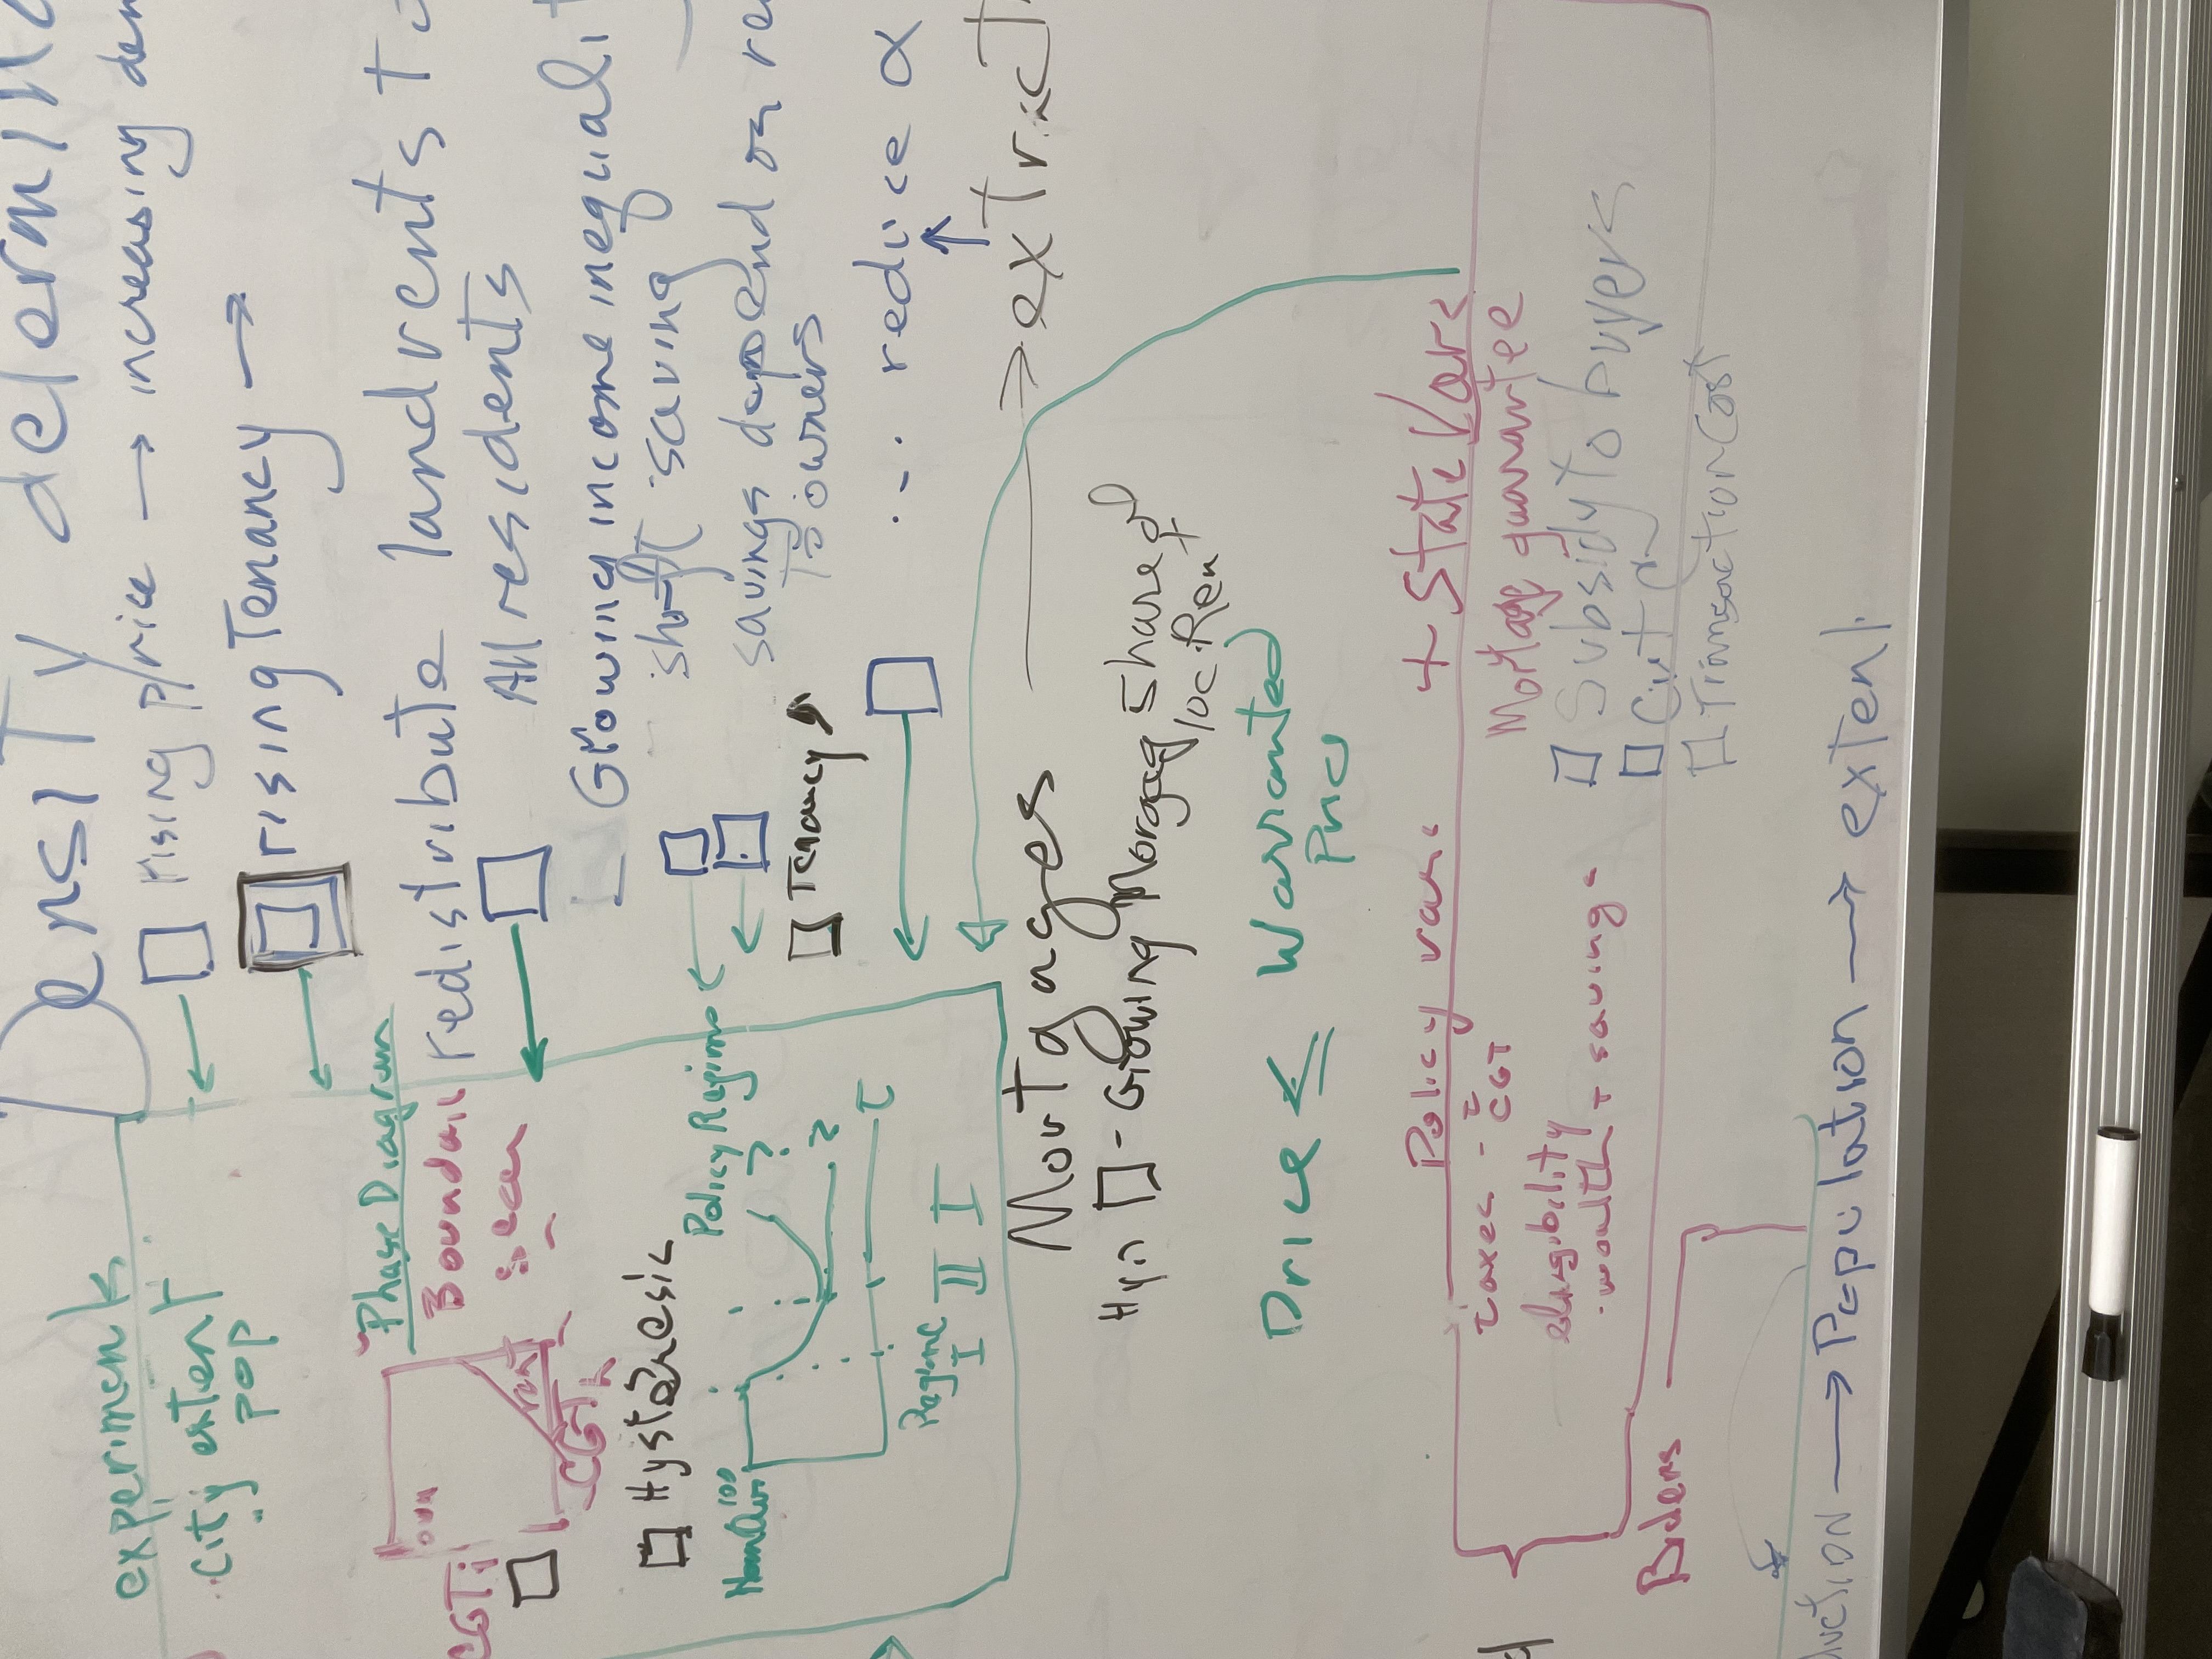
\includegraphics[scale=.5, angle=-90]{fig/IMG_2689.jpg} %Density determination

%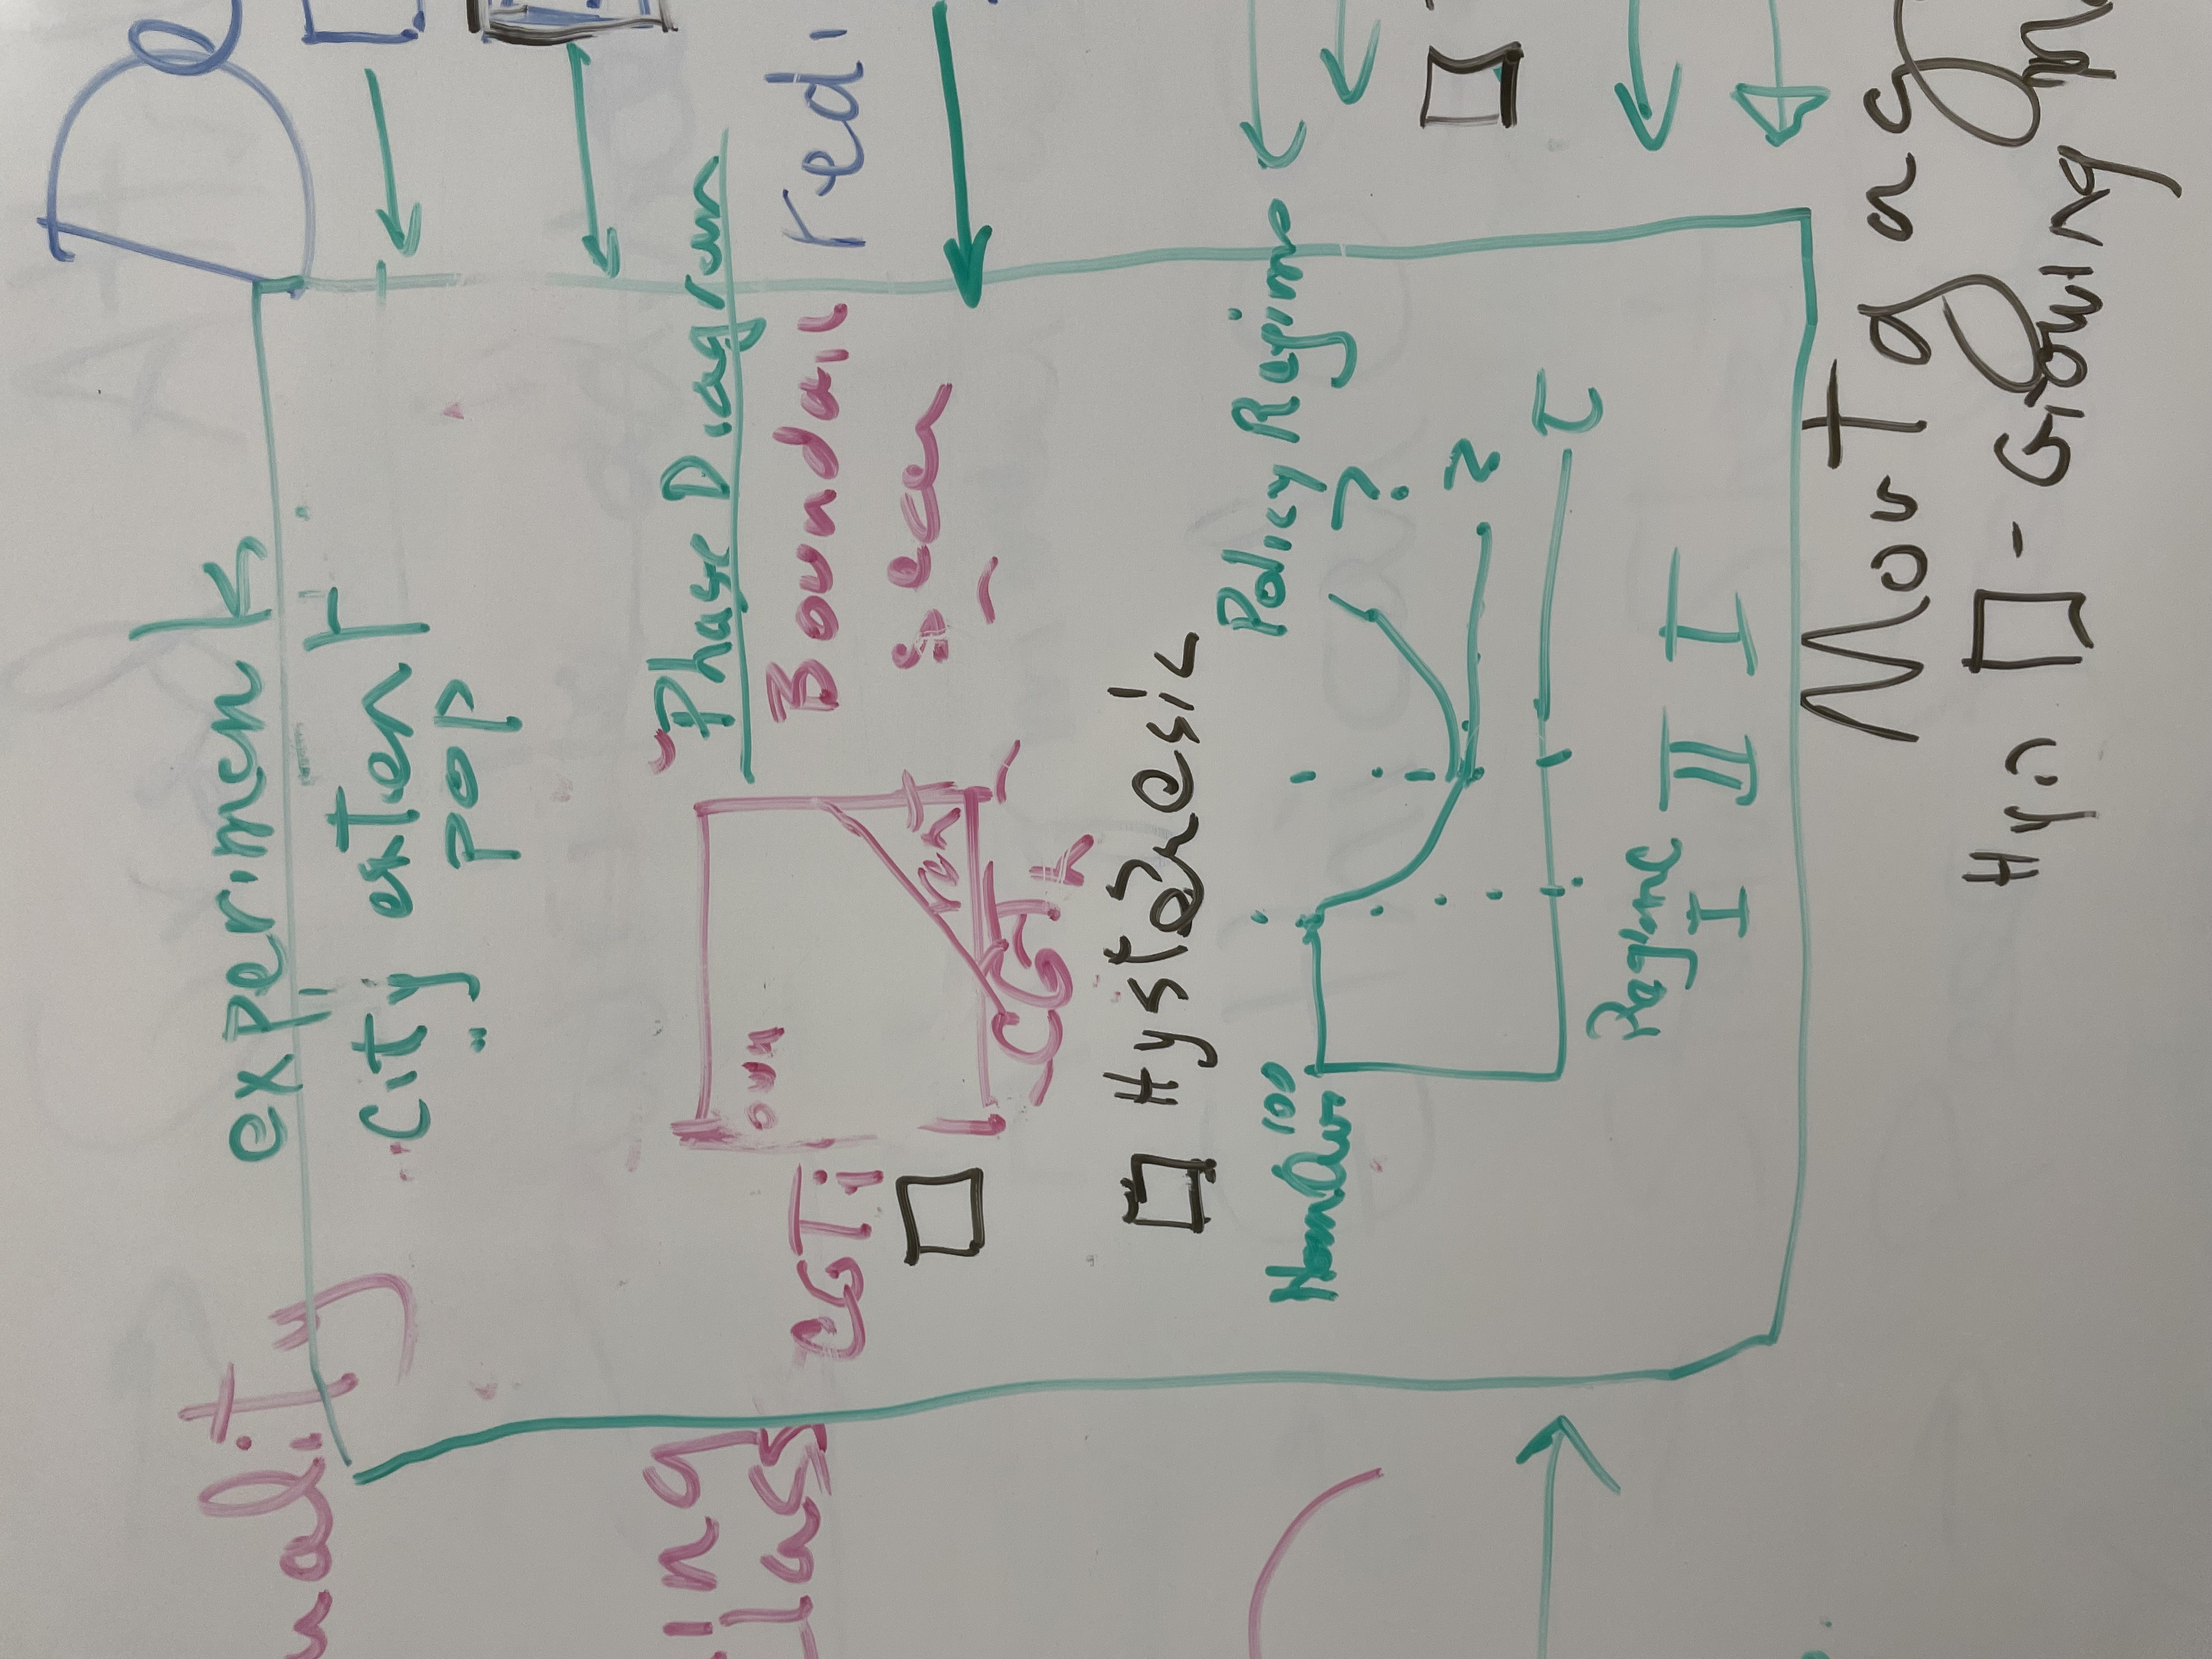
\includegraphics[scale=.5, angle=-90]{fig/IMG_2690.jpg}% 2 FIGURES NEEDED  
%$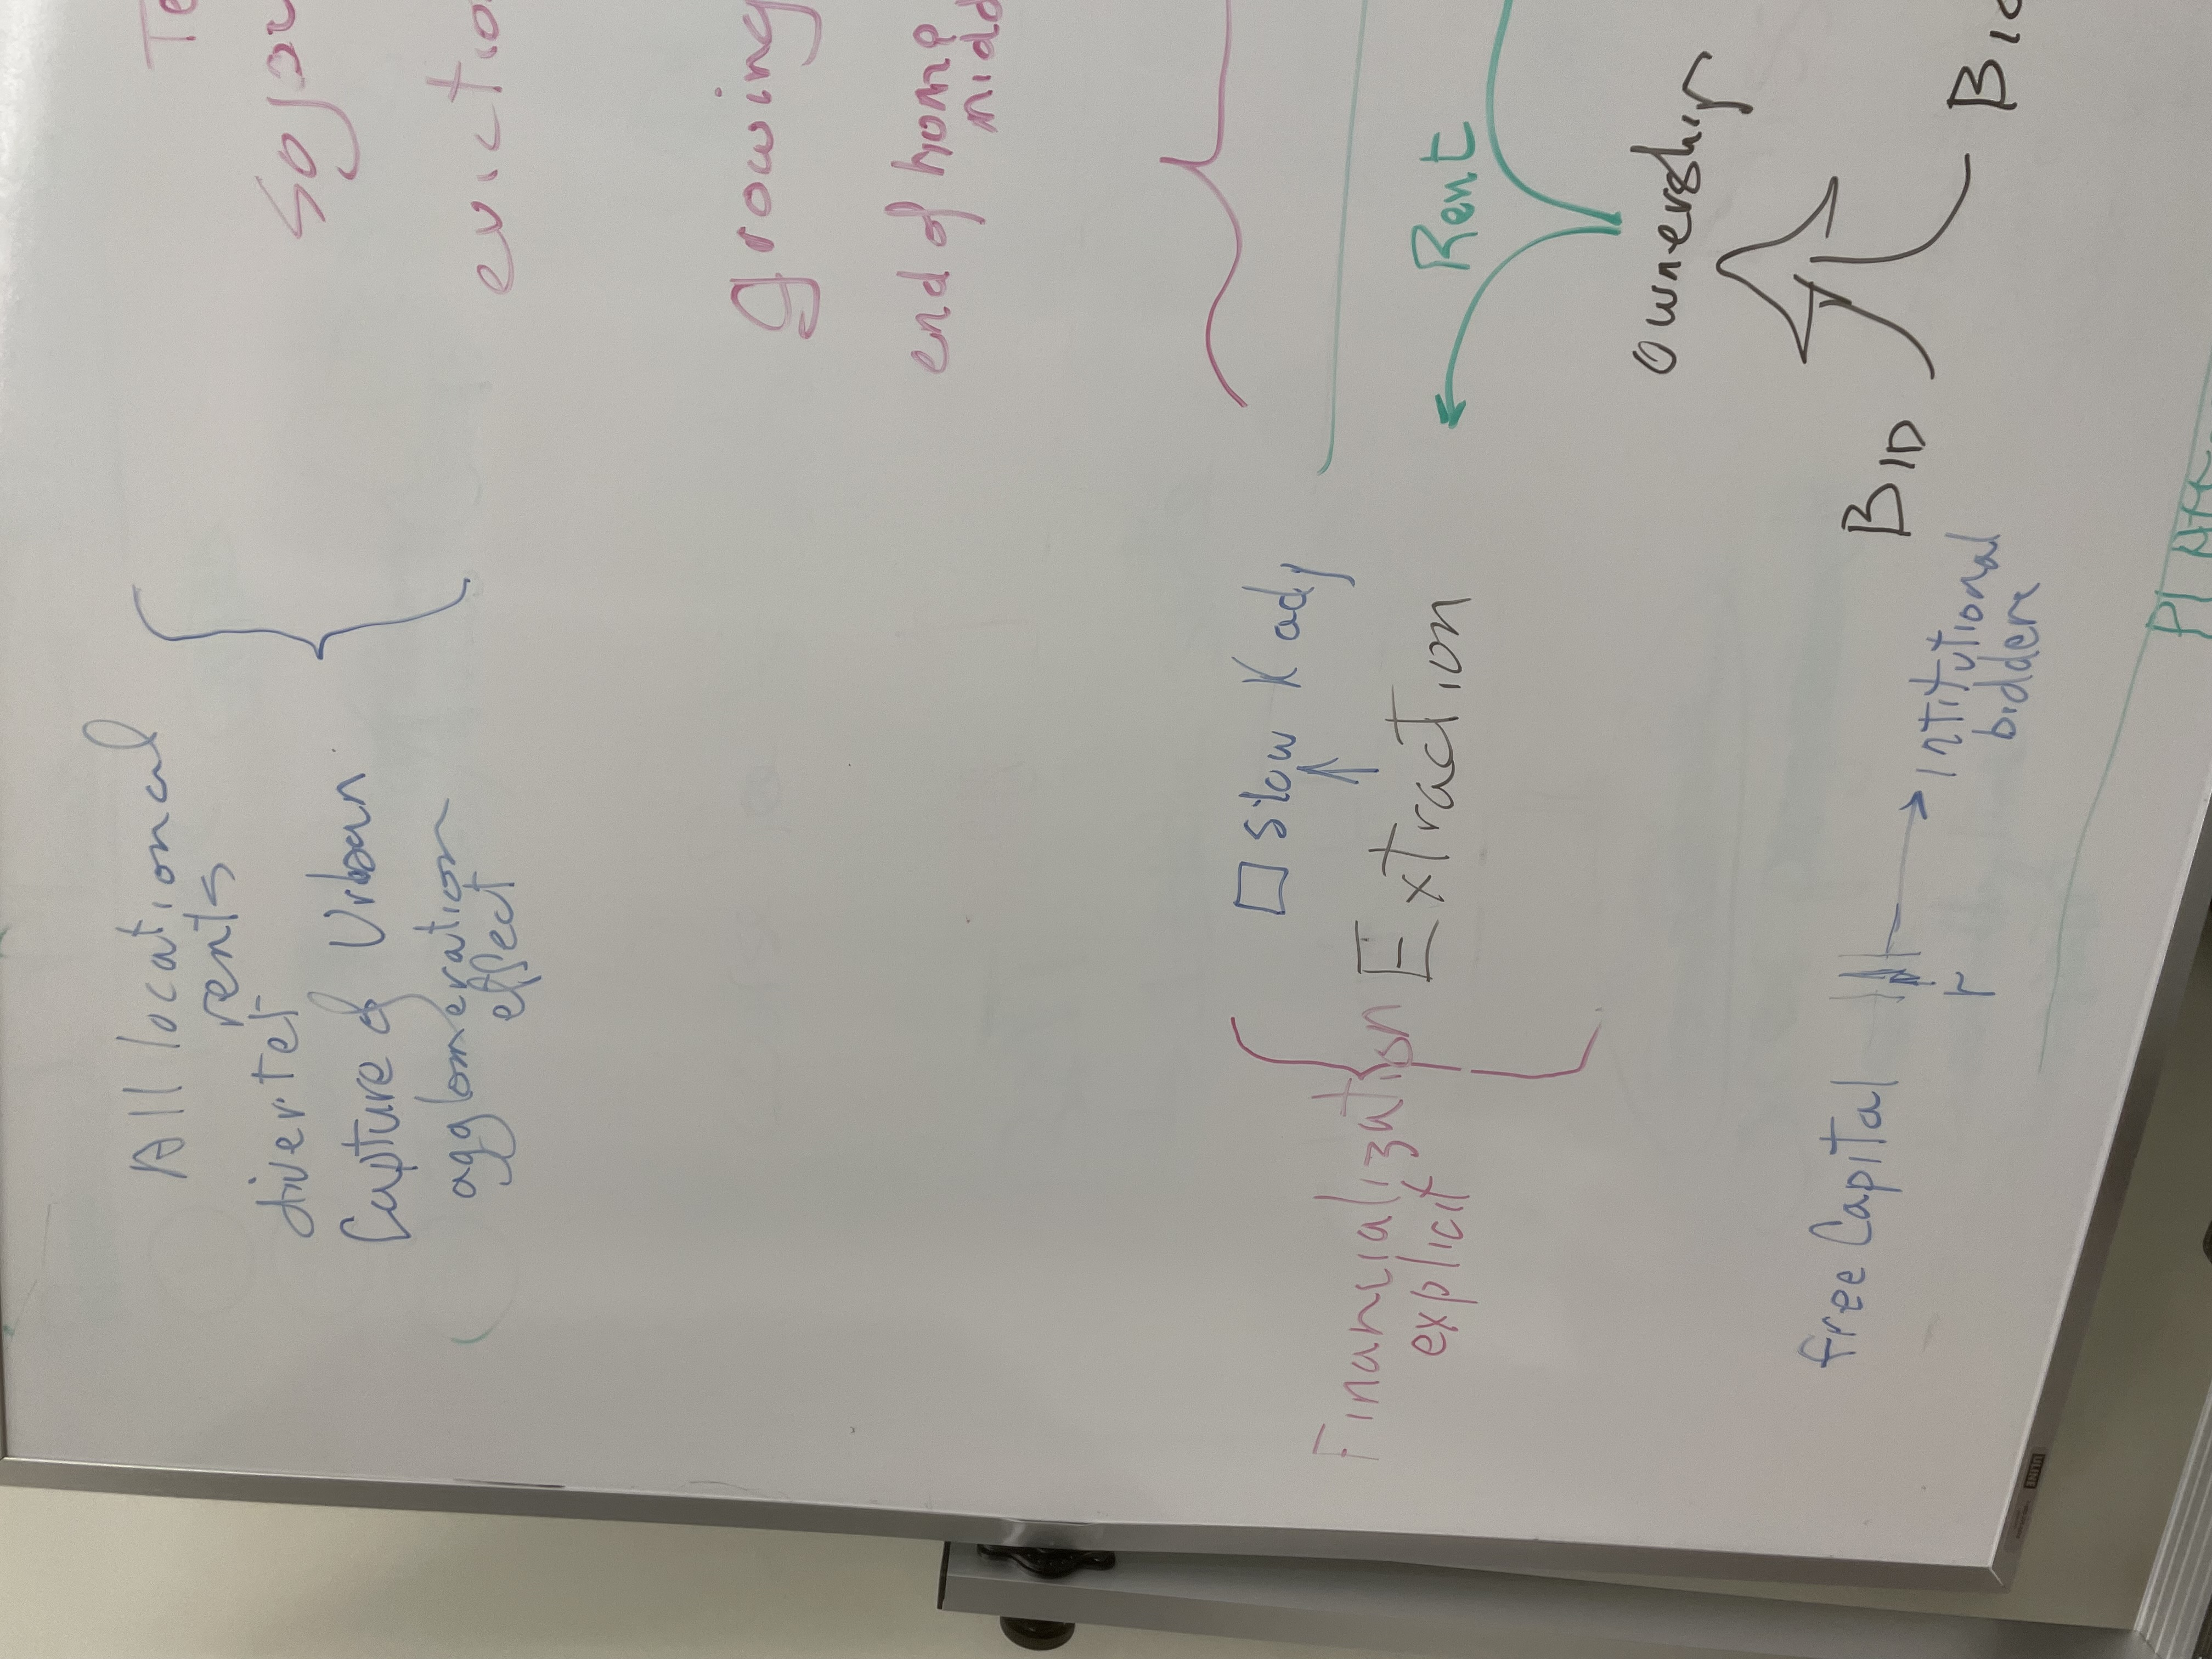
\includegraphics[scale=.5, angle=-90]{fig/IMG_2692.jpg}

To illustrate a decline in investment we can reduce Kadj.

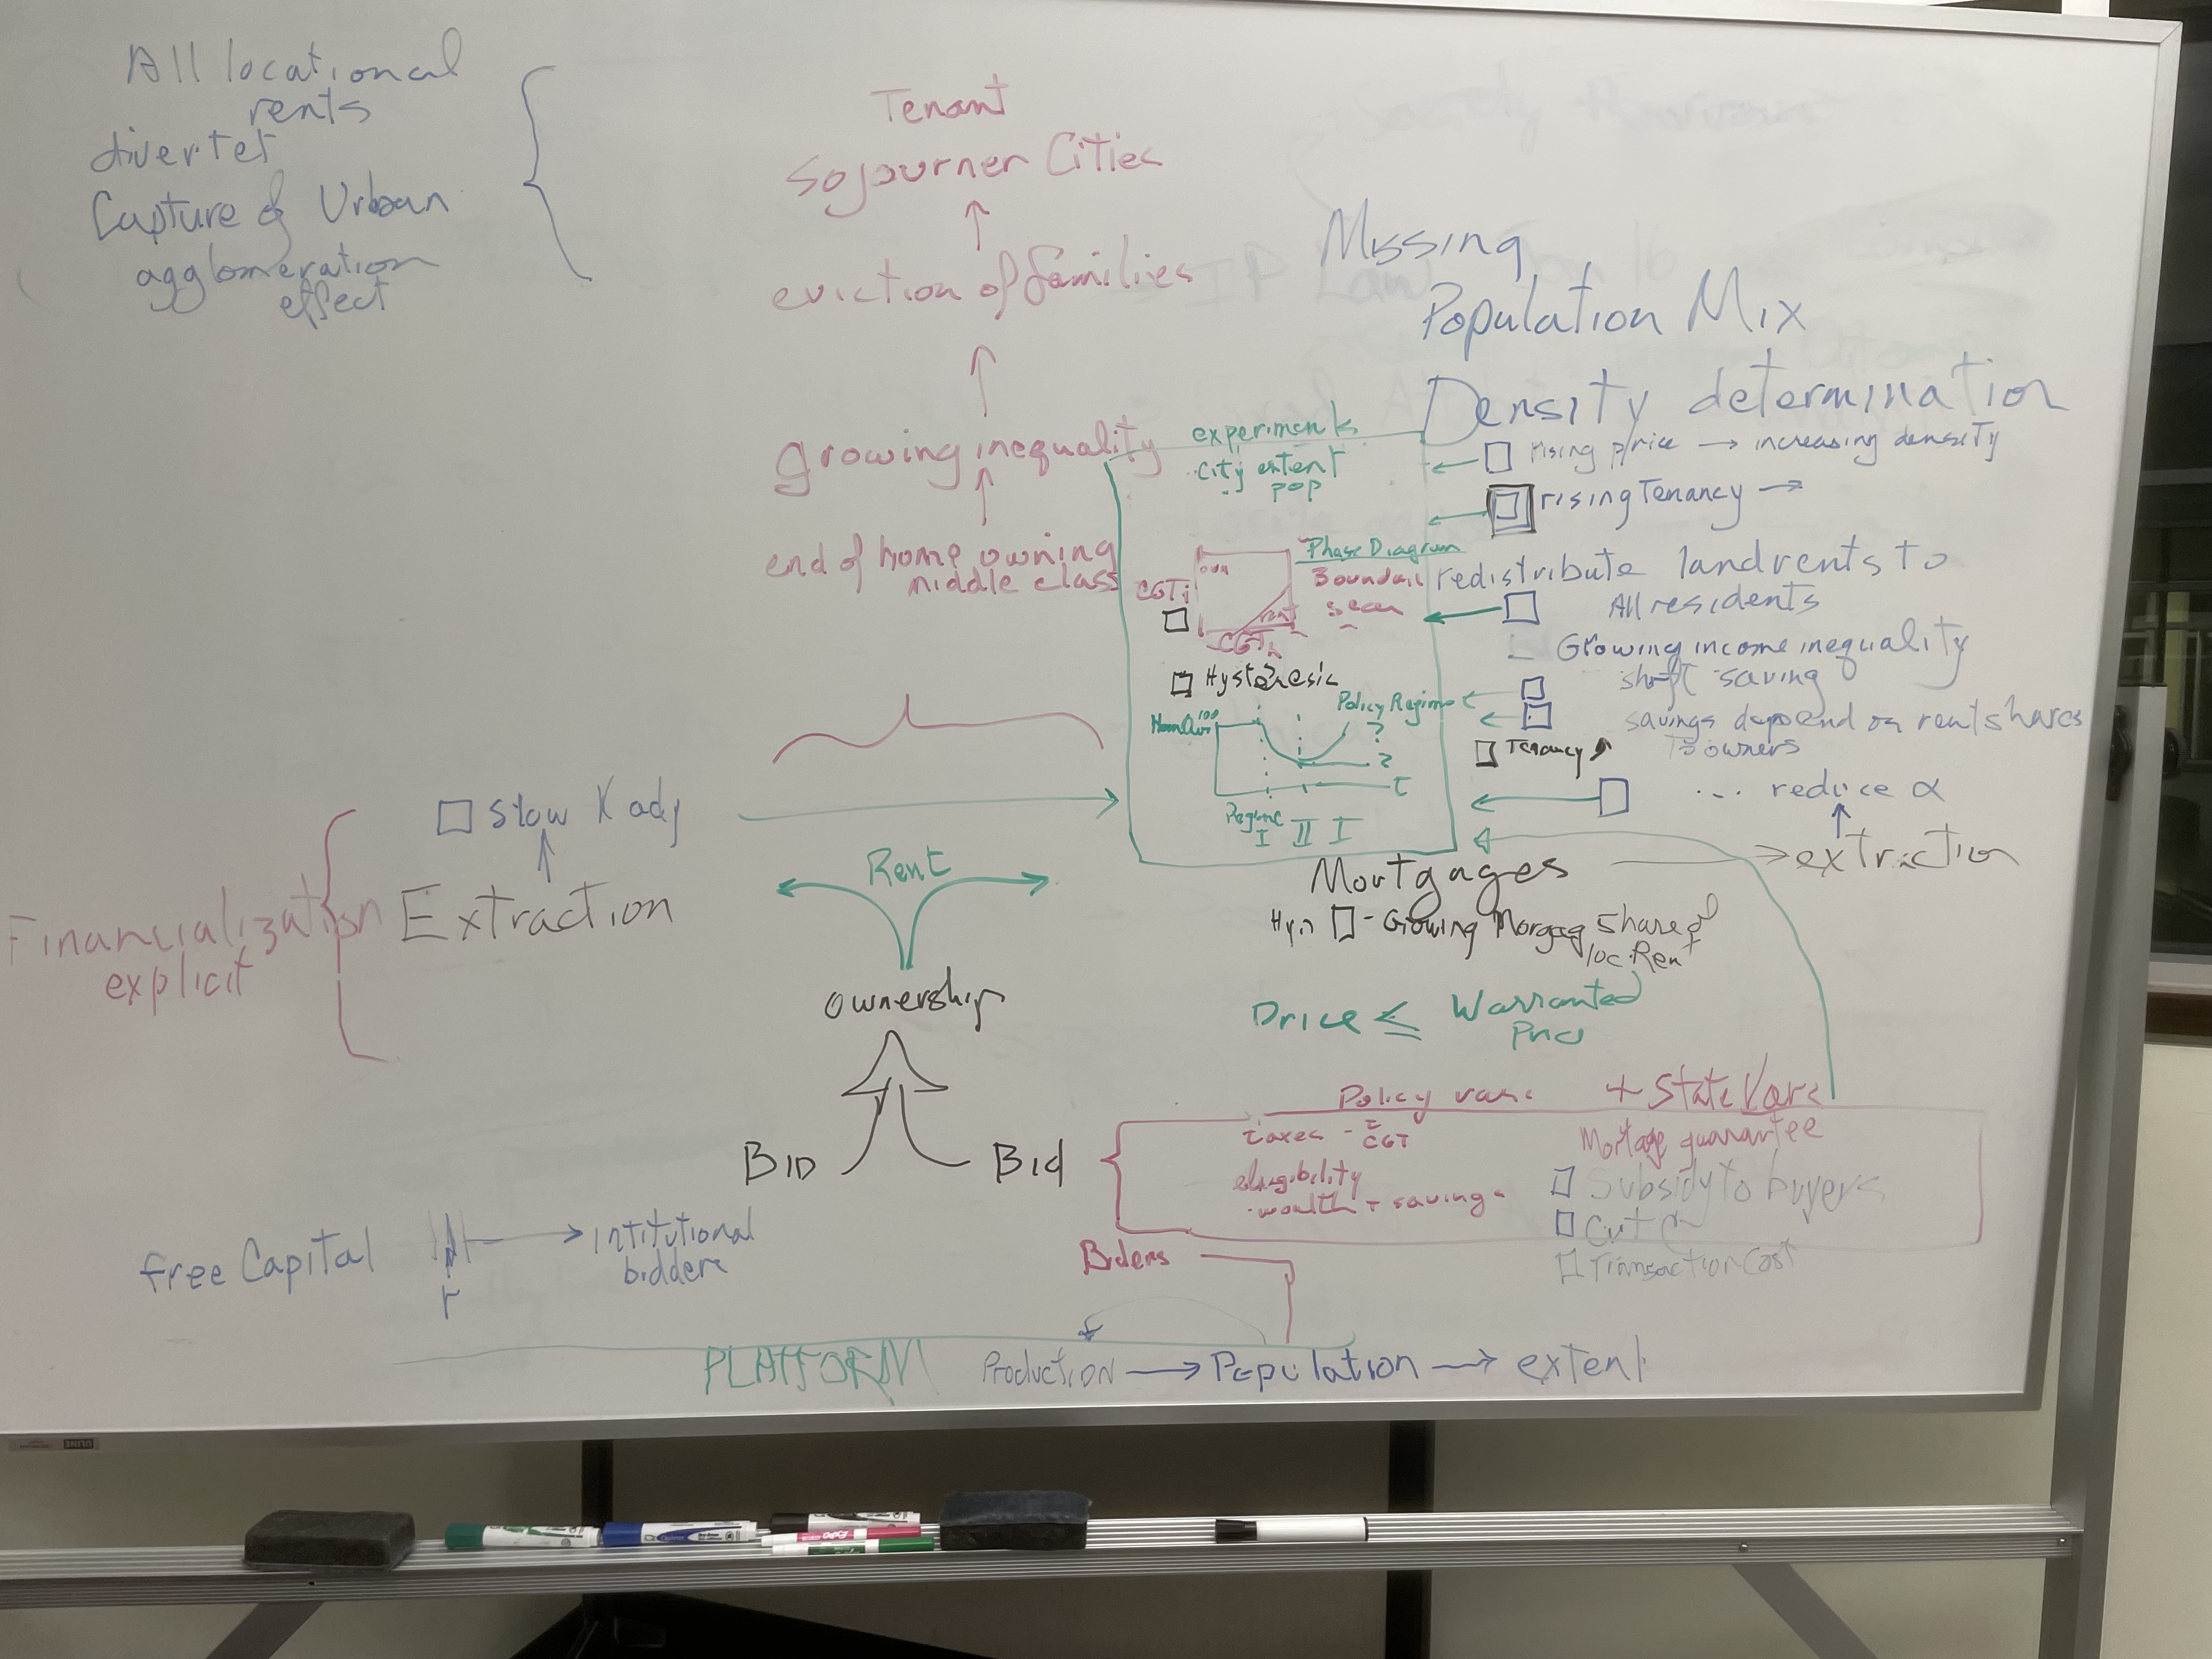
\includegraphics[scale=.5]{fig/IMG_2693.jpg}



Initially, 100\% of locational land rent accrues to residents. In the end, 100\% accrues to the owners of financial capital. Total rents at the end of the period of growth are eight times their initial size.\footnote{Recall that the radius of a circular city is proportional to the wage premium. Rent can be visualized as a cone of volume $\pi r^2 h$ where $h$ is the wage premium. If we double $h$, the volume is increased by a factor of 8.}



 \section{Implications for urban productivity}

 To explore the impact of financialization on productivity we introduce explicit links between ownership and .productivity